

% ==========================================================================================
% 
%                                     LFC ERRORS
% 
% ==========================================================================================
\section{LFC photon count errors}\label{appendix:LFC_errors} 

\begin{SCfigure}[1][!ht]%
    \begin{wide}  
    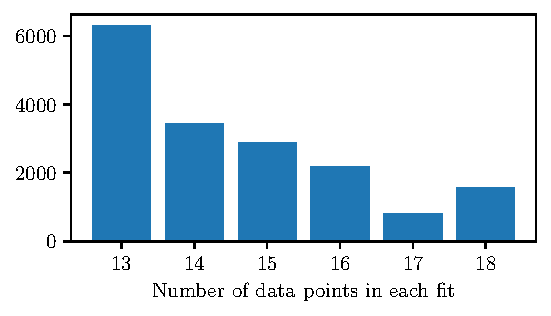
\includegraphics[scale=1]{figures/N_data_points.pdf}
    \caption{Number of data points in each LFC peak fit, determined by the average distance between peaks in each order.}
    \label{fig:N_data_points}
\end{wide}
\end{SCfigure}


\begin{SCfigure}[1][!ht]%
    \begin{wide}  
    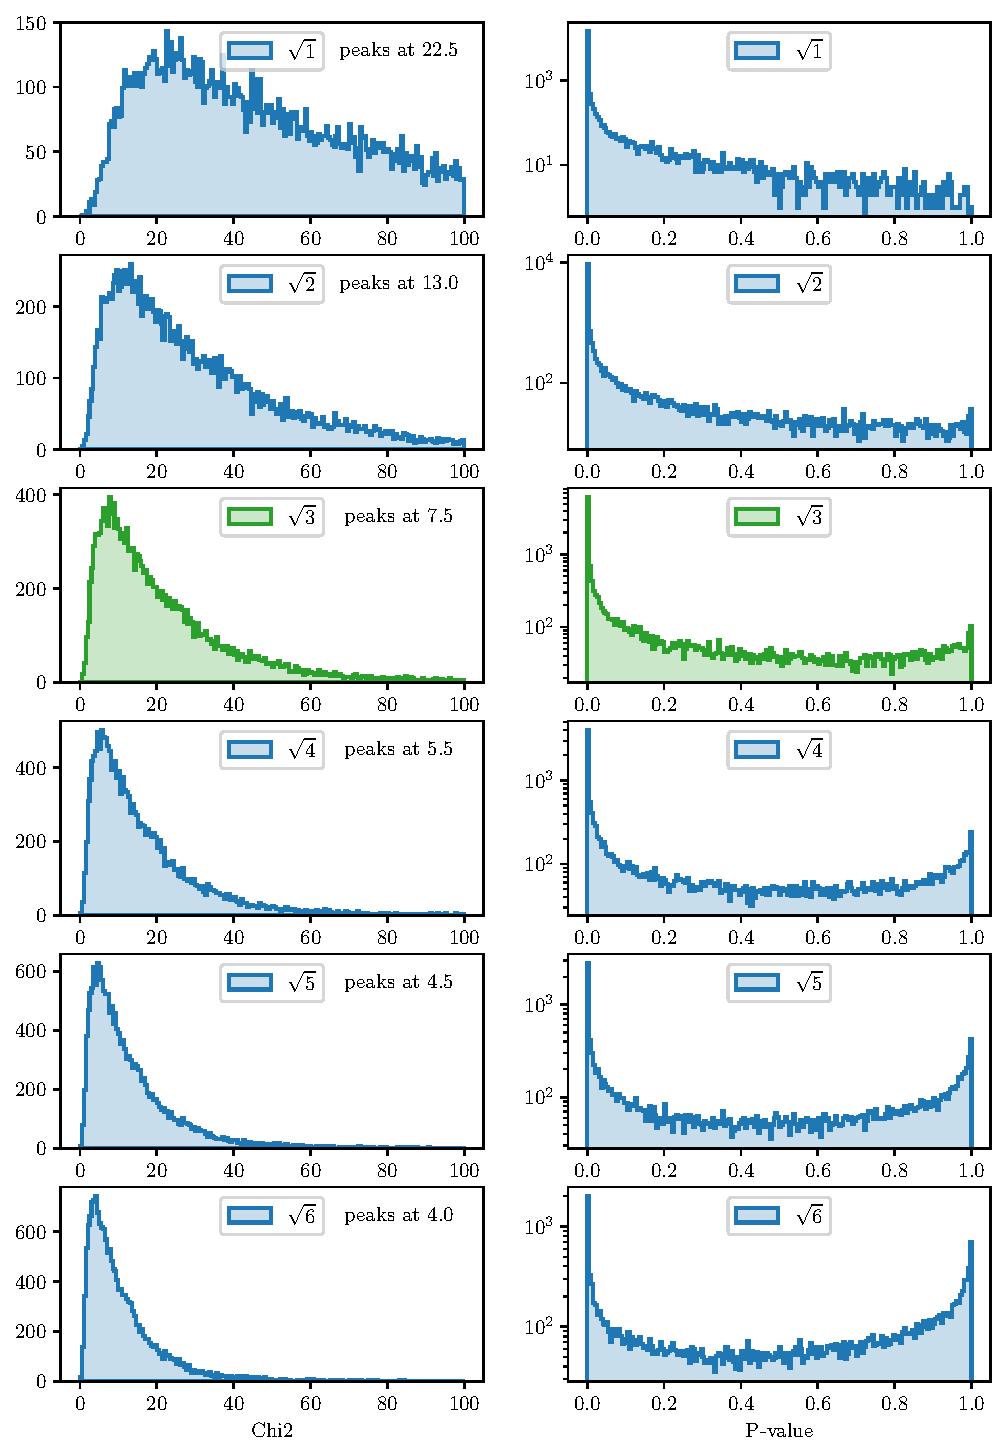
\includegraphics[scale=0.72]{figures/calib_errors_extensive.pdf}
    \caption{Chi2-values and P-values from individual LFC peak super-gauss fits with photon count (spectrum) errors multiplied by different scale-factors.}
    \label{fig:calib_errors_extensive}
\end{wide}
\end{SCfigure}




% ==========================================================================================
% 
%                                     RV EXTRACTIONS
% 
% ==========================================================================================
\newpage
\section{RV extractions}\label{appendix:RV_extraction}

\begin{SCfigure}[1][!ht]%
    \begin{wide}  
    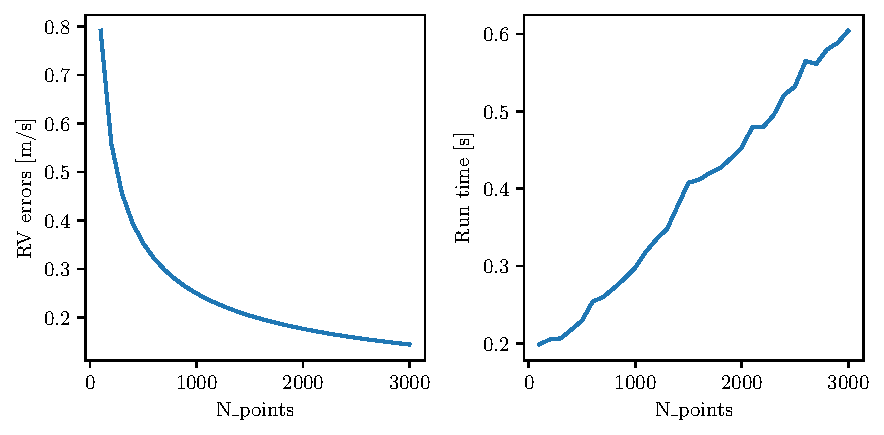
\includegraphics[scale=0.72]{figures/err_vs_run_time.pdf}
    \caption{Number of data points in each LFC peak fit, determined by the average distance between peaks in each order.}
    \label{fig:err_vs_run_time}
\end{wide}
\end{SCfigure}

% \begin{figure}[ht]
%     \centering
%     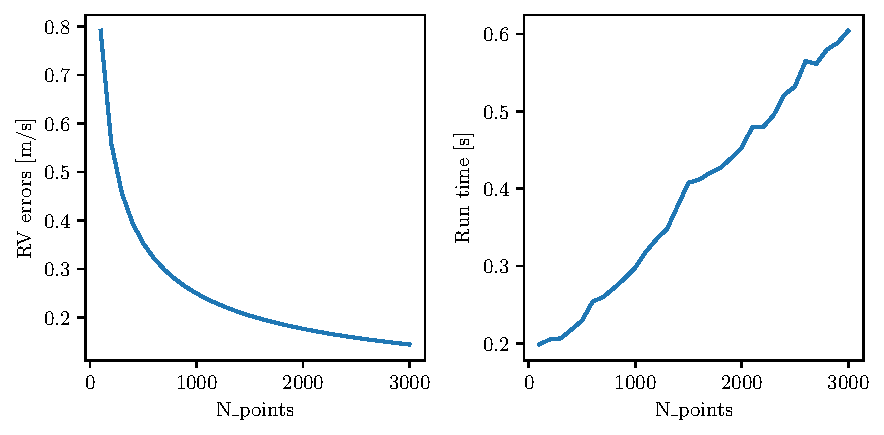
\includegraphics[scale=0.80]{figures/err_vs_run_time.pdf}
%     \caption{Number of data points in each LFC peak fit, determined by the average distance between peaks in each order.}
%     \label{fig:err_vs_run_time}
% \end{figure}


